%In this section, the layer is described in some detail in terms of its specific subsystems. Describe each of the layers and its subsystems in a separate chapter/major subsection of this document. The content of each subsystem description should be similar. Include in this section any special considerations and/or trade-offs considered for the approach you have chosen.
Groco is to use a relational database to keep backend information uniform and well structured.  The database will not maintain any information gathered from grocery searches.  Since such information would become obsolete so quickly, the userbase would have to become rather large for the hit rate of such a cache to make it worth having.  Furthermore, since the collection of such data is in its own subsystem, the integration of such a cache later on would require relatively little more work than would be required to have it added intially, thus, it is better to leave such a system for future analysis and upgrades.  Note that the following subsections reference figure \ref{fig:db.1}, but this figure is only shown once in subsection \ref{section:db.1} to avoid being verbose.


\subsection{UserTable Subsystem}\label{section:db.1}
The UserTable Subsystem will be used for storing identifiable information about each user and holding information to help the user.

\begin{figure}[h!]\label{fig:db.1}
	\centering
 	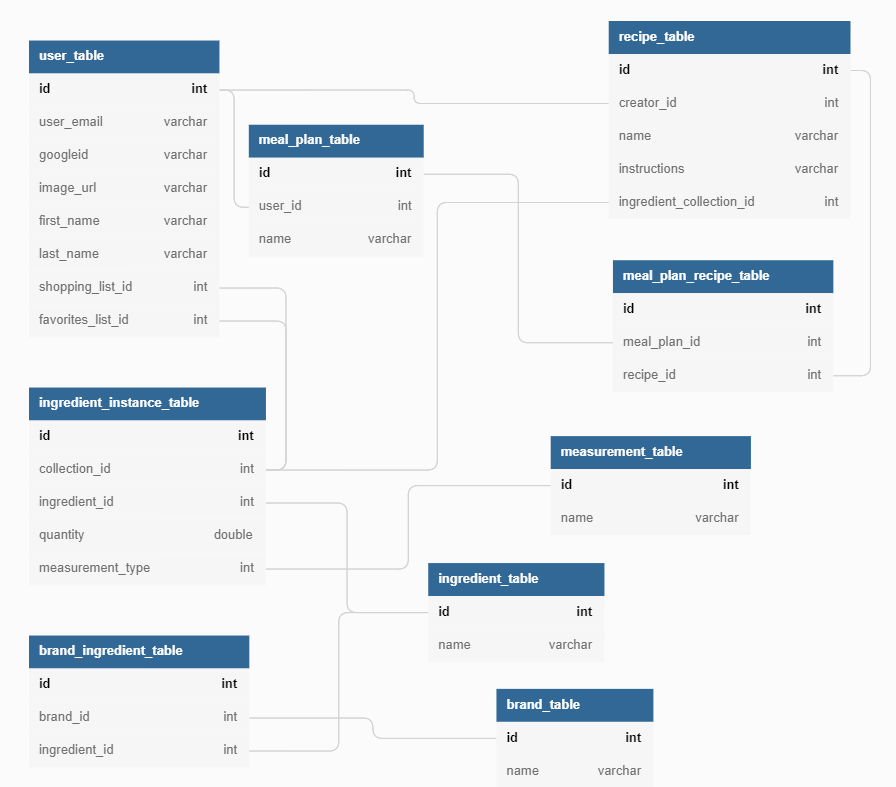
\includegraphics[width=0.60\textwidth]{images/databasenew.png}
 \caption{Database Diagram}
\end{figure}

\subsubsection{Assumptions}
The users google ID, profile picture and Name shall be needed and stored in the database.

\subsubsection{Responsibilities}
Whenever a user is added to the system, their email, username, and password will be added to this table.  A global ID will also be used to improve data efficiency and ensure data integrity.  Their password is also stored as a hash instead of plain form for better security, but this field may end up being removed if it is proven obsolete by other authentication systems such as AWS authentication.  A few other noteworthy fields in this table are are "shopping\_list\_id" and "favorites\_list\_id" which point to the current shopping list and favorite items list, which will be discussed in subsection \ref{section:db.3}.

%Each of the responsibilities/features/functions/services of the subsystem as identified in the architectural summary must be expanded to more detailed responsibilities. These responsibilities form the basis for the identification of the finer-grained responsibilities of the layer's internal subsystems. Clearly describe what each subsystem does.

\subsubsection{Subsystem Interfaces}
%Each of the inputs and outputs for the subsystem are defined here. Create a table with an entry for each labelled interface that connects to this subsystem. For each entry, describe any incoming and outgoing data elements will pass through this interface.
\begin {table}[H]
\caption {Subsystem interfaces} 
\begin{center}
    \begin{tabular}{ | p{1cm} | p{6cm} | p{3cm} | p{3cm} |}
    \hline
    ID & Description & Inputs & Outputs \\ \hline
    \#1 & A new user entry is created & Username, password hash, and email & success/failure  \\ \hline
    \#2 & A user entry is updated & A field of "UserTable" is updated for a particular given user ID. & success/failure  \\ \hline
    \#3 & A user entry is deleted & A user ID & success/failure  \\ \hline
    \#4 & A user is queried & username/email, hashed password & user record  \\ \hline
    \end{tabular}
\end{center}
\end{table}


\subsection{Meal Plan Subsystem}\label{section:db.2}
The Meal Plan Subsystem will be incharge of complying with customer requirements regarding having meal plans and related features.

%\begin{figure}[h!]\label{fig:db.1}
%	\centering
% 	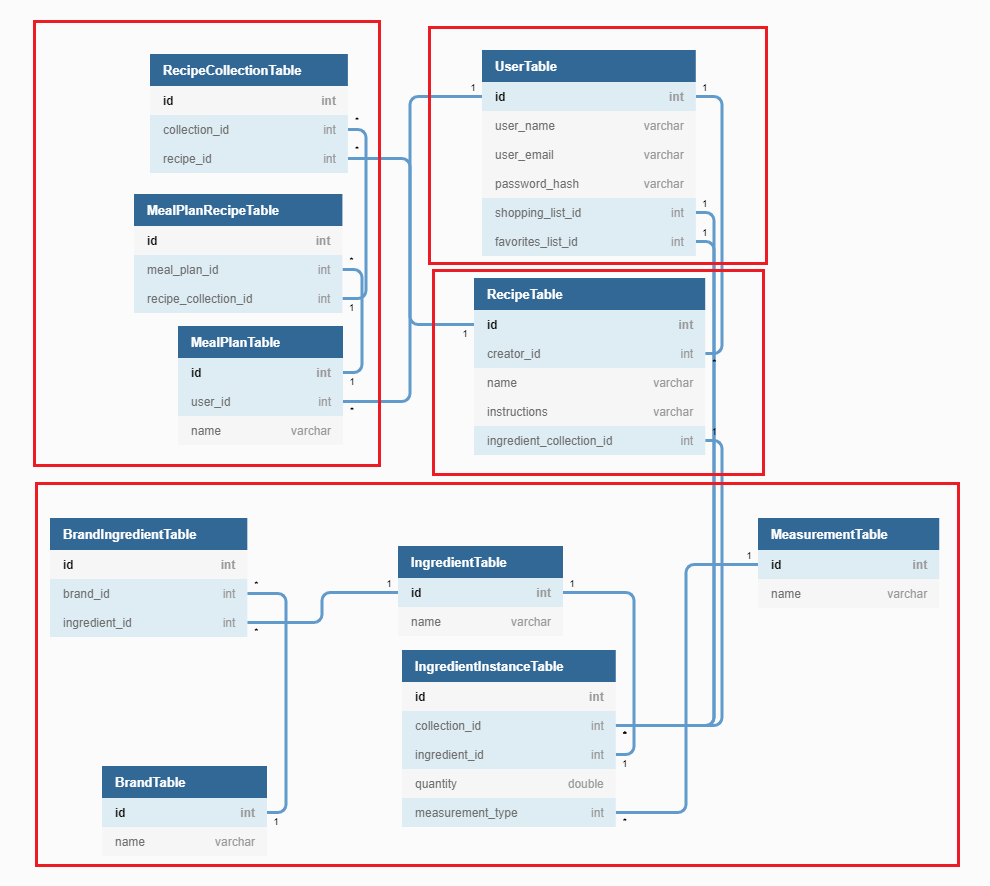
\includegraphics[width=0.60\textwidth]{images/Database}
% \caption{Database Diagram}
%\end{figure}

\subsubsection{Assumptions}
There are no assumptions for this subsystem.
%The users email and password shall be needed and stored in the database.

\subsubsection{Responsibilities}
%Storing identifiable information about each user and holding information to help the user.
%Each of the responsibilities/features/functions/services of the subsystem as identified in the architectural summary must be expanded to more detailed responsibilities. These responsibilities form the basis for the identification of the finer-grained responsibilities of the layer's internal subsystems. Clearly describe what each subsystem does.
For meal plans, several layers of one to many relationships are needed.  Consider the following enumeration to get an idea of those:
\begin{enumerate}
    \item To allow the user to have multiple meal plans, "MealPlanTable" maps each user ID to zero or more meal plans, each of which have their own name.
    \item To allow each meal plan to have multiple recipes, "MealPlanRecipeTable" maps each meal plan to zero or more recipes.
\end{enumerate}

\subsubsection{Subsystem Interfaces}
\begin {table}[H]
\caption {Subsystem interfaces} 
\begin{center}
    \begin{tabular}{ | p{1cm} | p{6cm} | p{3cm} | p{3cm} |}
    \hline
    ID & Description & Inputs & Outputs \\ \hline
    \#01 & A new meal plan is created & user ID, meal plan name & meal plan ID  \\ \hline
    \#02 & A meal plan is updated & A field of from the meal plan and the meal plan ID & success/failure  \\ \hline
    \#03 & A meal plan is deleted & meal plan ID & success/failure  \\ \hline
    \#04 & A recipe is added to a meal plan & meal plan ID, recipe ID & success/failure  \\ \hline
    \#05 & A recipe is removed to a meal plan & meal plan ID, recipe ID & success/failure  \\ \hline
    \#06 & A list of meal plans is queried & A user ID & A list of meal plans  \\ \hline
    \#07 & A list of meal recipes is queried & A meal plan ID & A list of recipes  \\ \hline
    \end{tabular}
\end{center}
\end{table}


\subsection{Ingredient Subsystem}\label{section:db.3}
The Ingredients Subystem will be used for storing ingredients used elsewhere in the database.

%\begin{figure}[h!]\label{fig:db.1}
%	\centering
% 	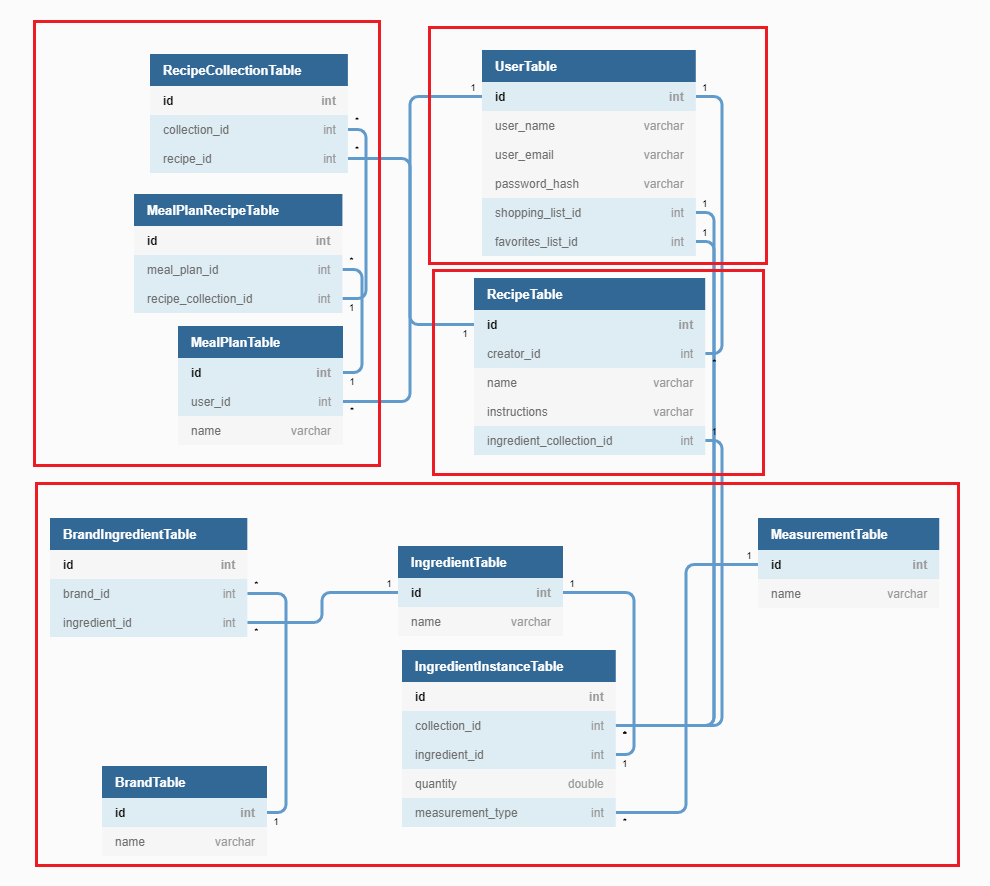
\includegraphics[width=0.60\textwidth]{images/Database}
% \caption{Database Diagram}
%\end{figure}

\subsubsection{Assumptions}
Whenever a shopping, favorites list, or recipe is cleared, the corrosponding collection ID will be discarded so that only ones in use will appear in "IngredientsInstanceTable".
%The users email and password shall be needed and stored in the database.

\subsubsection{Responsibilities}
The system needs to be able to know the names of ingredients and the amounts needed for shopping lists and recipes.  These two needs are met by "IngredientTable" and "IngredientInstanceTable" respectively.  The former mearly holds the name of each ingredient, which can be used to comply with the grocery search requirements mentioned in the SRS.  The latter is a bit more complicated, the various fields are broken down in the following list:
\begin{itemize}
    \item id: Global id for each enty to ensure uniqueness, this may end up being removed if shown unneeded.
    \item collection\_id: Every user shopping list, user favorites list, and recipe will have an associated collection id, which will corrospond to everything on that list.  Each of those items for that "collection" will fall in this table.  By constructing the database in this way, several requirements are satisfied with a single table.
    \item quantity: Gives the amount required of the ingredient in the units specified in the next field.
    \item measurement\_type: Has a key corrosponding to the particular measurement type in use.
\end{itemize}

%Each of the responsibilities/features/functions/services of the subsystem as identified in the architectural summary must be expanded to more detailed responsibilities. These responsibilities form the basis for the identification of the finer-grained responsibilities of the layer's internal subsystems. Clearly describe what each subsystem does.

\subsubsection{Subsystem Interfaces}
\begin {table}[H]
\caption {Subsystem interfaces} 
\begin{center}
    \begin{tabular}{ | p{1cm} | p{6cm} | p{3cm} | p{3cm} |}
    \hline
    ID & Description & Inputs & Outputs \\ \hline
    \#01 & An ingredient instance is added & ingredient ID, measurement ID, amount, collection ID & particular ingredient ID  \\ \hline
    \#02 & An ingredient instance is updated & particular ingredient ID, other field value & success/failure  \\ \hline
    \#03 & An ingredient instance is deleted & particular ingredient ID & success/failure  \\ \hline
    \#04 & An unused collection ID is requested & none & the largest collection ID currently in use in the table  \\ \hline
    \end{tabular}
\end{center}
\end{table}

\subsection{RecipeTable Subsystem}\label{section:db.4}
The RecipeTable Subsystem will responsible maintaining lists of all recipes, along with associated ingredient collection IDs.

%\begin{figure}[h!]\label{fig:db.1}
%	\centering
% 	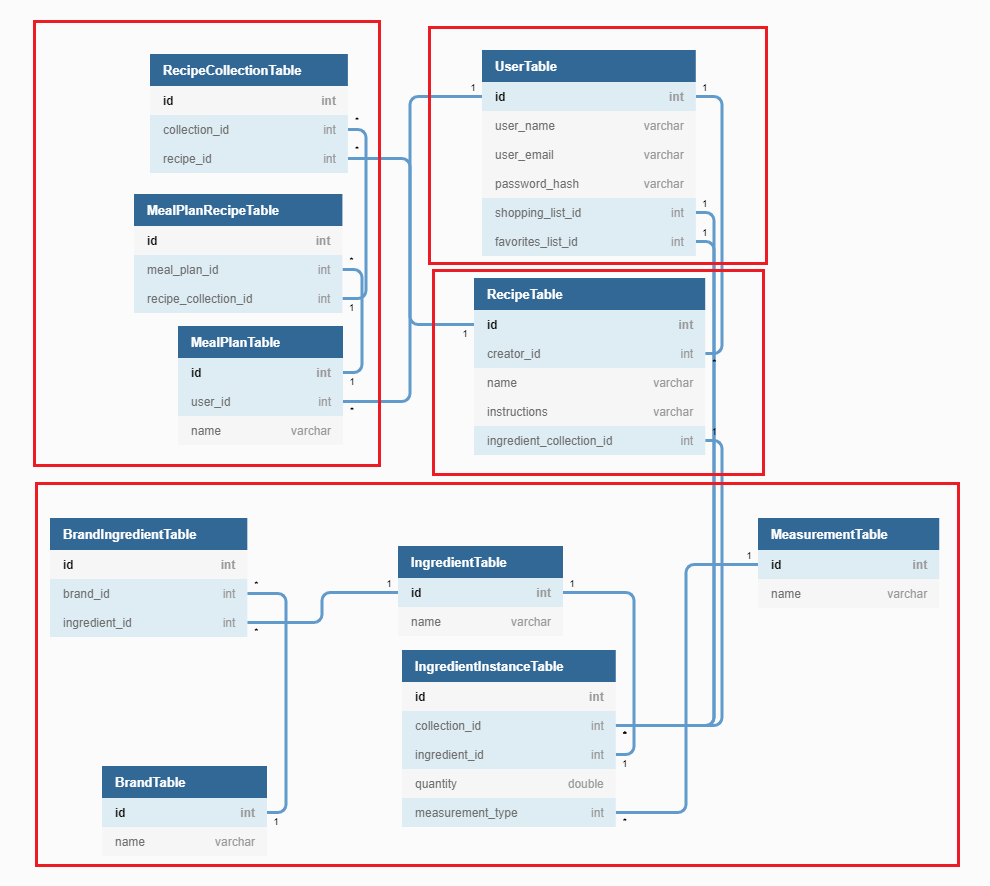
\includegraphics[width=0.60\textwidth]{images/Database}
% \caption{Database Diagram}
%\end{figure}

\subsubsection{Assumptions}
Any recipe can be written as a set of instructions and ingredients.

\subsubsection{Responsibilities}
A table containing each recipe within the application.  The first few fields are fairly straightforward, giving a unique ID to each recipe, the ID of the creature of the recipe, the name of the recipe, and instructions on how to make the recipe.  The last field, as discussed in subsection \ref{section:db.3}, gives the ID which can be used to query the particular ingredients for the recipe.  This last field is to be used in constructing shopping lists.

%Each of the responsibilities/features/functions/services of the subsystem as identified in the architectural summary must be expanded to more detailed responsibilities. These responsibilities form the basis for the identification of the finer-grained responsibilities of the layer's internal subsystems. Clearly describe what each subsystem does.

\subsubsection{Subsystem Interfaces}
\begin {table}[H]
\caption {Subsystem interfaces} 
\begin{center}
    \begin{tabular}{ | p{1cm} | p{6cm} | p{3cm} | p{3cm} |}
    \hline
    ID & Description & Inputs & Outputs \\ \hline
    \#01 & A recipe is added & all field values except ID & recipe ID  \\ \hline
    \#02 & A recipe is updated & recipe ID, other field value & success/failure  \\ \hline
    \#03 & A recipe is deleted & recipe ID & success/failure  \\ \hline
    \end{tabular}
\end{center}
\end{table}